\documentclass[]{book}
\usepackage{lmodern}
\usepackage{amssymb,amsmath}
\usepackage{ifxetex,ifluatex}
\usepackage{fixltx2e} % provides \textsubscript
\ifnum 0\ifxetex 1\fi\ifluatex 1\fi=0 % if pdftex
  \usepackage[T1]{fontenc}
  \usepackage[utf8]{inputenc}
\else % if luatex or xelatex
  \ifxetex
    \usepackage{mathspec}
  \else
    \usepackage{fontspec}
  \fi
  \defaultfontfeatures{Ligatures=TeX,Scale=MatchLowercase}
\fi
% use upquote if available, for straight quotes in verbatim environments
\IfFileExists{upquote.sty}{\usepackage{upquote}}{}
% use microtype if available
\IfFileExists{microtype.sty}{%
\usepackage{microtype}
\UseMicrotypeSet[protrusion]{basicmath} % disable protrusion for tt fonts
}{}
\usepackage{hyperref}
\hypersetup{unicode=true,
            pdftitle={10X Transcriptomic Data Cloud Processing},
            pdfauthor={Ho Lab},
            pdfborder={0 0 0},
            breaklinks=true}
\urlstyle{same}  % don't use monospace font for urls
\usepackage{natbib}
\bibliographystyle{apalike}
\usepackage{longtable,booktabs}
\usepackage{graphicx,grffile}
\makeatletter
\def\maxwidth{\ifdim\Gin@nat@width>\linewidth\linewidth\else\Gin@nat@width\fi}
\def\maxheight{\ifdim\Gin@nat@height>\textheight\textheight\else\Gin@nat@height\fi}
\makeatother
% Scale images if necessary, so that they will not overflow the page
% margins by default, and it is still possible to overwrite the defaults
% using explicit options in \includegraphics[width, height, ...]{}
\setkeys{Gin}{width=\maxwidth,height=\maxheight,keepaspectratio}
\IfFileExists{parskip.sty}{%
\usepackage{parskip}
}{% else
\setlength{\parindent}{0pt}
\setlength{\parskip}{6pt plus 2pt minus 1pt}
}
\setlength{\emergencystretch}{3em}  % prevent overfull lines
\providecommand{\tightlist}{%
  \setlength{\itemsep}{0pt}\setlength{\parskip}{0pt}}
\setcounter{secnumdepth}{5}
% Redefines (sub)paragraphs to behave more like sections
\ifx\paragraph\undefined\else
\let\oldparagraph\paragraph
\renewcommand{\paragraph}[1]{\oldparagraph{#1}\mbox{}}
\fi
\ifx\subparagraph\undefined\else
\let\oldsubparagraph\subparagraph
\renewcommand{\subparagraph}[1]{\oldsubparagraph{#1}\mbox{}}
\fi

%%% Use protect on footnotes to avoid problems with footnotes in titles
\let\rmarkdownfootnote\footnote%
\def\footnote{\protect\rmarkdownfootnote}

%%% Change title format to be more compact
\usepackage{titling}

% Create subtitle command for use in maketitle
\providecommand{\subtitle}[1]{
  \posttitle{
    \begin{center}\large#1\end{center}
    }
}

\setlength{\droptitle}{-2em}

  \title{10X Transcriptomic Data Cloud Processing}
    \pretitle{\vspace{\droptitle}\centering\huge}
  \posttitle{\par}
    \author{Ho Lab}
    \preauthor{\centering\large\emph}
  \postauthor{\par}
      \predate{\centering\large\emph}
  \postdate{\par}
    \date{2019-11-27}

\usepackage{booktabs}

\begin{document}
\maketitle

{
\setcounter{tocdepth}{1}
\tableofcontents
}
\hypertarget{prerequisites}{%
\chapter{Prerequisites}\label{prerequisites}}

\textbf{1. Amazon Web Services (AWS) Account:}

Create free Amazon Web Services (AWS) Account

\url{https://portal.aws.amazon.com/billing/signup?redirect_url=https\%3A\%2F\%2Faws.amazon.com\%2Fregistration-confirmation\#/start}

\textbf{2. Command Line Interface (CLI):}

MacOS or Linux Operating System.

\textbf{For Windows Users:}
Install Windows Subsystem for Linux

\url{https://docs.microsoft.com/en-us/windows/wsl/install-win10}

\hypertarget{intro}{%
\chapter{Introduction}\label{intro}}

Amazon Web Services provides cloud computing capabilities, which allows on-demand compute power, database, storage, applications, and other IT resources via the internet. This allows extremely flexibile and customisable of usage of their products depending on your specific demands/requirements.

This could be in the form of computing power, i.e.~CPU cores and memory, or data storage space. All requested resources from AWS can be rescaled for your business operations, thus optimising efficiency and cost savings. Set up and usage is also extremely fast and simple, available for usage for all user background types.

In this workshop, we will exploit AWS's cloud computing service, Elastic Compute Cloud (EC2), to perform single cell 10X genomics RNA-sequencing data processing. Specifically, the mapping of raw transcript reads to an annotated human genome, which is generally a computationally demanding task, requiring more than 32GBs of RAM and numerous threads for efficient/timely processing.

10X genomics single cell RNA-sequencing (scRNA-seq) technology is becoming the most predominant type of scRNA-seq performed due to its high sequencing depth and library preparation technique to capture UMI/cell barcodes. This technology has enabled sequencing on the scale of thousands to millions of individual cells, which generates raw data files much larger than previous bulk sequencing experiements. For this reason, the average local computer generally does not hold enough computing power to perform analysis on this big data.

\begin{verbatim}
**Quiz**
1. What are UMIs and cell barcodes? and why are they beneficial?
2. What format are raw transcript reads stored as? 
(a) Fasta (b) Fastq (c) Fastx (d) BAM (e) SAM
3. Estimate the file size of 
(a) Raw transcript file
(b) Aligned reads file (binary compressed format)
(c) Feature count matrix
\end{verbatim}

\hypertarget{aws-ec2-instance}{%
\chapter{AWS EC2 Instance}\label{aws-ec2-instance}}

\hypertarget{introduction}{%
\section{Introduction}\label{introduction}}

An AWS EC2 instance is equivalent to a portable, customisable, intangible computer which is accessible through your personal local computer with a command line interface. We are able to specify memory requirements, CPU power (computing cores/threads), data storage size, and the operation system (e.g.~Linux, Ubuntu, Windows) of this intangible computer.

\hypertarget{set-up}{%
\section{Set Up}\label{set-up}}

\begin{enumerate}
\def\labelenumi{\arabic{enumi}.}
\item
  Log into your AWS Account.
\item
  Navigate to EC2 under Amazon's Services tab.
\item
  Select AMIs under IMAGES tab.
\item
  Change filter bar to ``Public Images'' and search for ``10X Workshop'' and launch.
\end{enumerate}

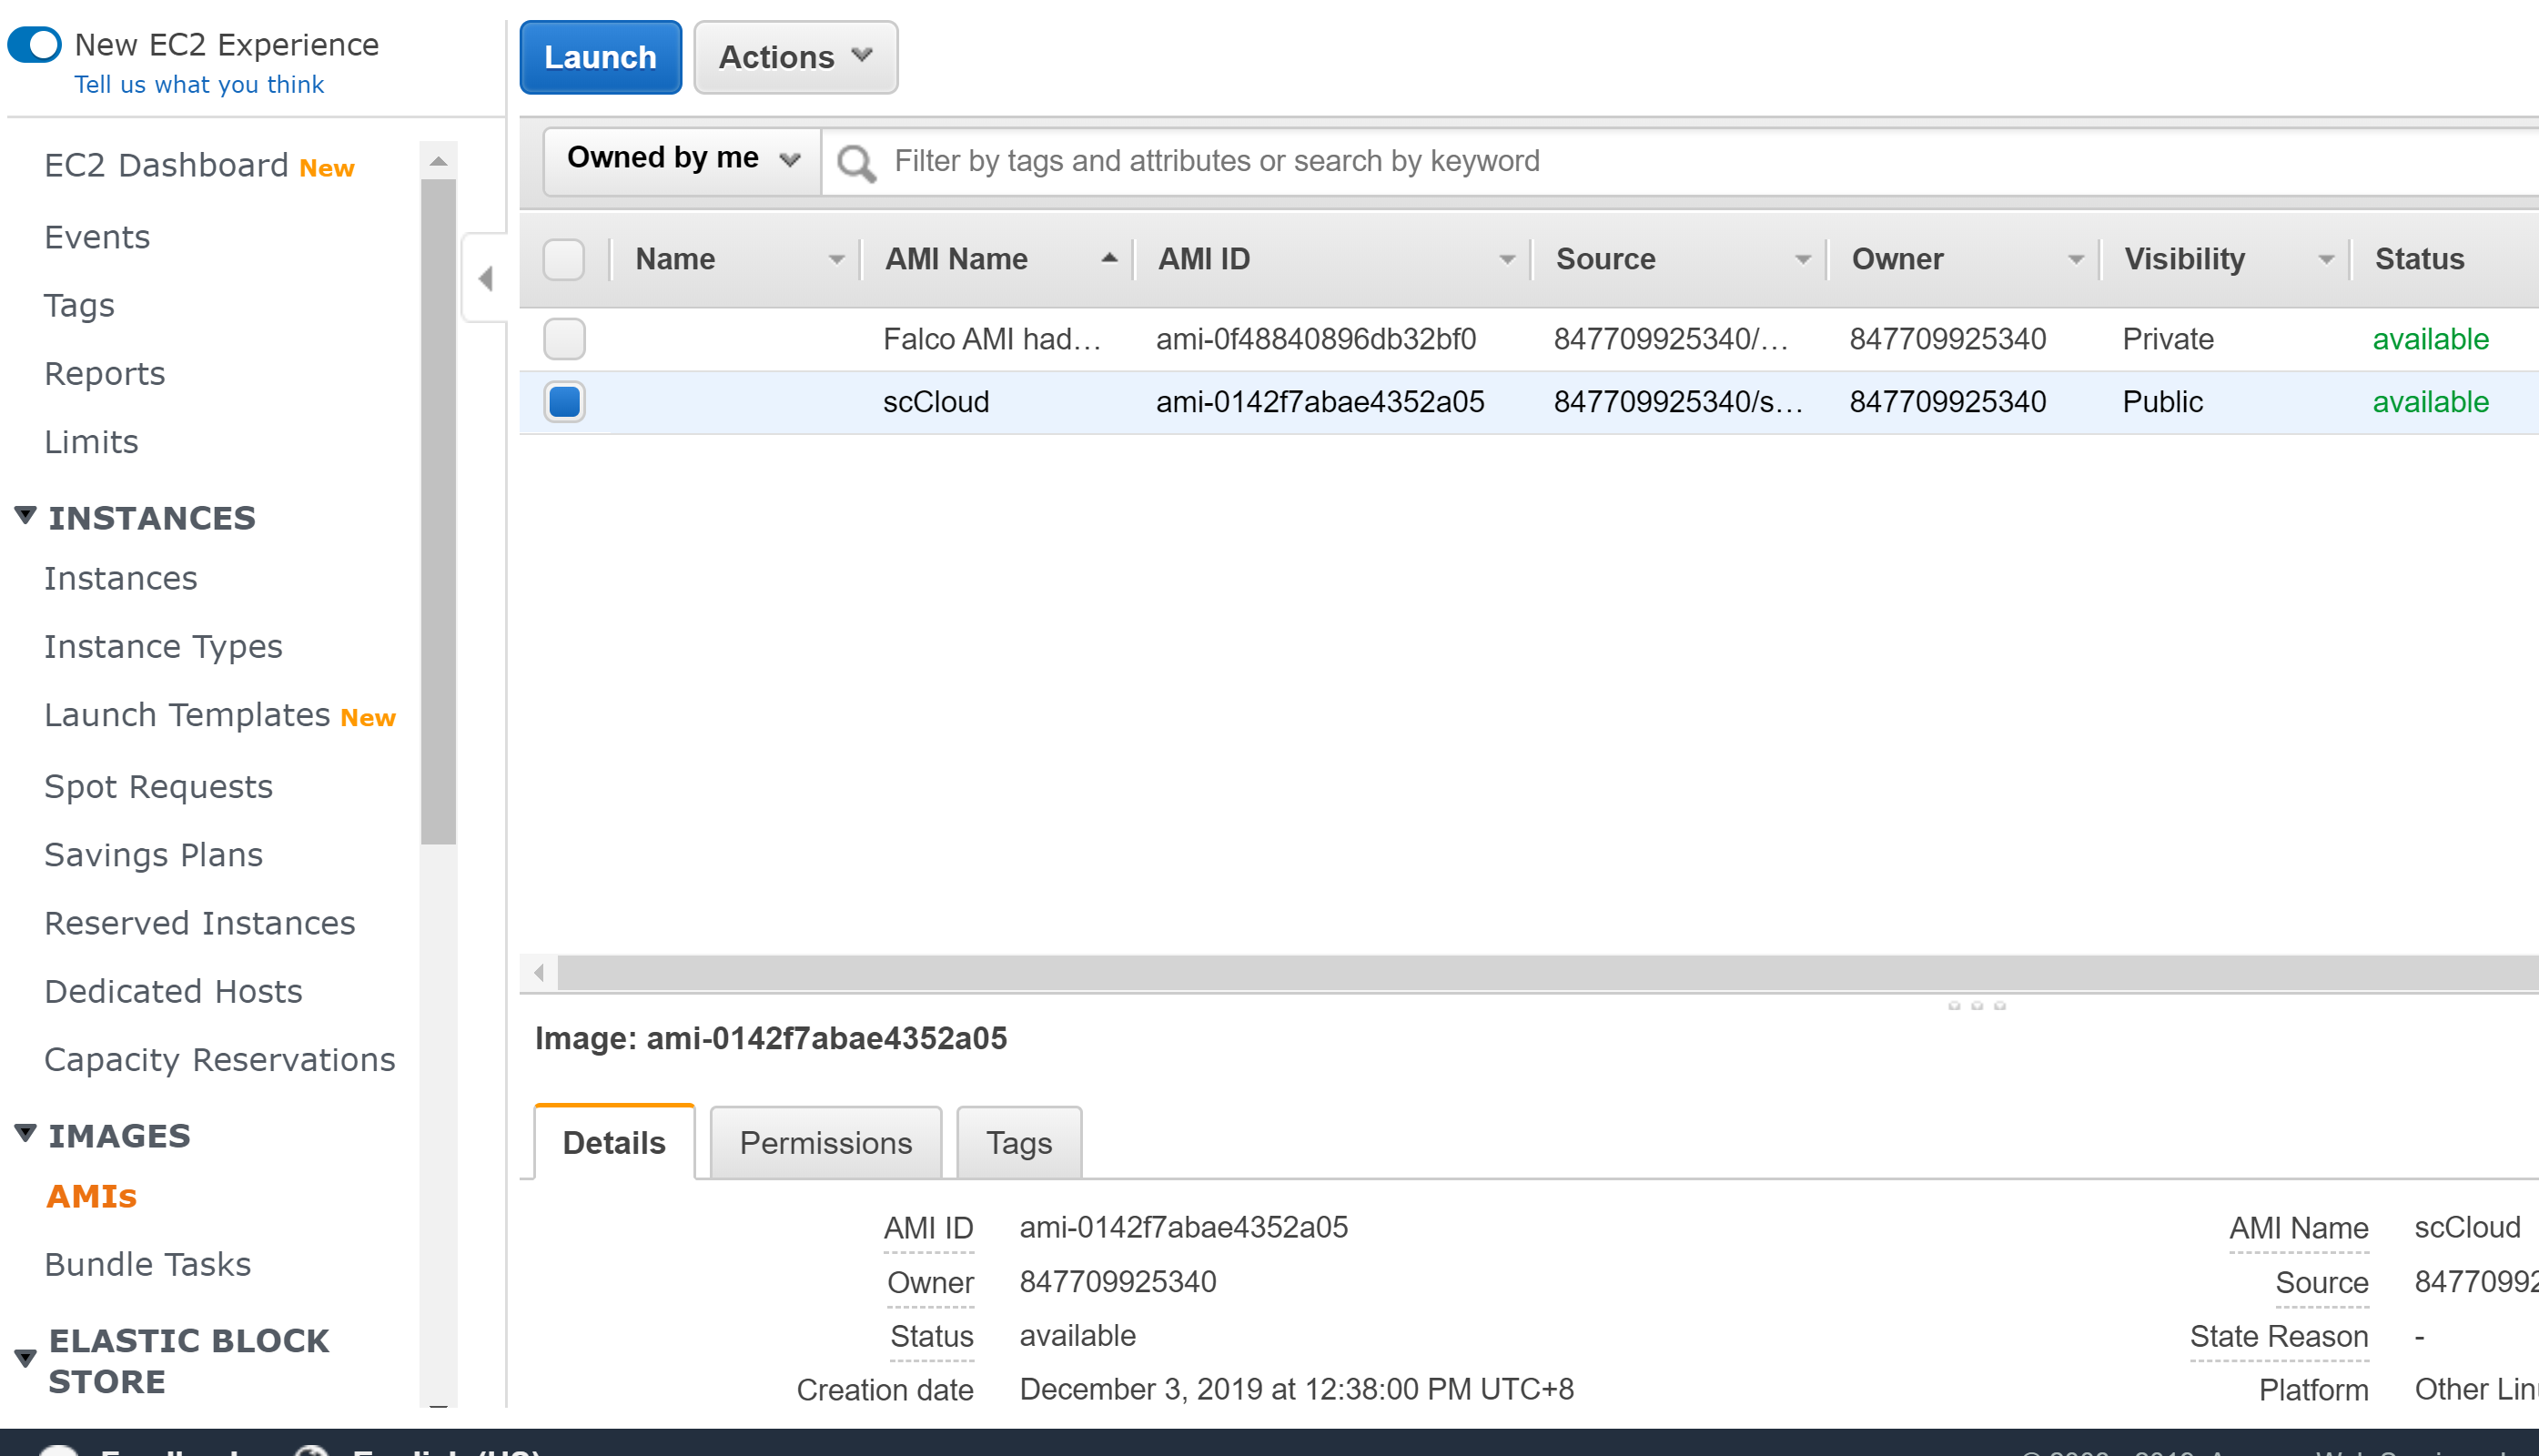
\includegraphics[width=26.61in]{_book/10X_files/figure-html/AMI}

\begin{enumerate}
\def\labelenumi{\arabic{enumi}.}
\setcounter{enumi}{3}
\item
  Launch specfication to use: \texttt{m5.4xlarge} instance type and \texttt{64GBs} of storage space. (Leave other options to default)
\item
  Click Launch.
\item
  When given the ``Key pair'' prompt: select ``Create a new key pair''. Name your key pair ``10X'' and download. Then ``Launch Instances''
\end{enumerate}

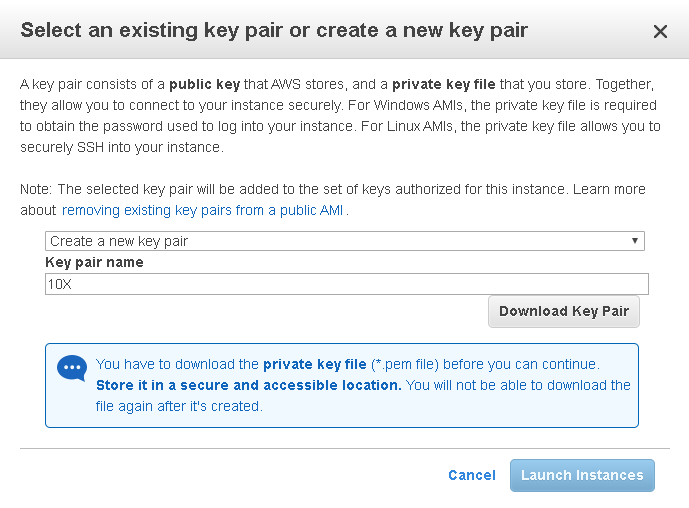
\includegraphics[width=6.89in]{_book/10X_files/figure-html/key_pair}

\begin{verbatim}
**Quiz**
1. What is an AMI?
2. What is the purpose of a key pair?
\end{verbatim}

\hypertarget{connecting-to-your-ec2-instance}{%
\section{Connecting to your EC2 instance}\label{connecting-to-your-ec2-instance}}

\begin{enumerate}
\def\labelenumi{\arabic{enumi}.}
\item
  Open your command line interface
\item
  Connect to your EC2 instance by entering the following command.
\end{enumerate}

\begin{verbatim}
ssh -i "10X.pem" ec2-user@ec2-XX-XXX-XX-XXX.ap-east-1.compute.amazonaws.com
\end{verbatim}

``10X.pem'' should be the location of where you have stored your key pair. The X's is the ip address of your personal EC2 instance. This can be found by going to EC2 Dashboard \textgreater{} Running Instances \textgreater{} Selecting your running instance \textgreater{} Click Connect.

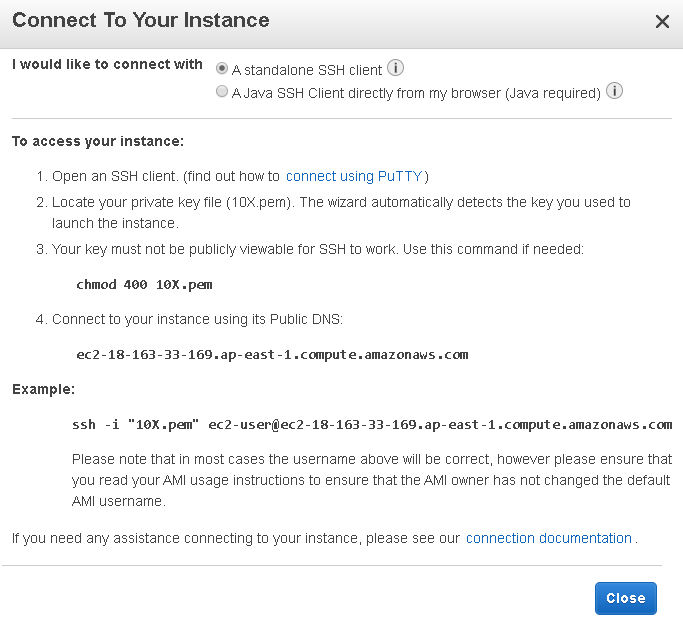
\includegraphics[width=6.83in]{_book/10X_files/figure-html/ec2}

\begin{enumerate}
\def\labelenumi{\arabic{enumi}.}
\setcounter{enumi}{2}
\tightlist
\item
  Type ``yes'' if prompted.
\end{enumerate}

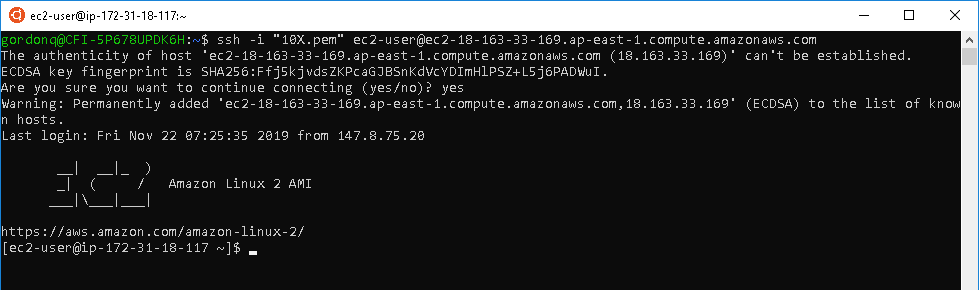
\includegraphics[width=9.79in]{_book/10X_files/figure-html/ssh}

\begin{verbatim}
**Quiz**
1. What is ssh?
\end{verbatim}

\hypertarget{processing-10x-rna-seq-data}{%
\chapter{Processing 10X RNA-seq data}\label{processing-10x-rna-seq-data}}

\hypertarget{introduction-1}{%
\section{Introduction}\label{introduction-1}}

Raw RNA-sequencing data will be in the format of a fastq file. This format describes the read ID, read sequence and sequencing quality scores. Represented in the following format:

\begin{verbatim}
>ReadID
READ SEQUENCE
+
SEQUENCING QUALITY SCORES
\end{verbatim}

Generally fastq files are pre-processed using quality control tools, such as FastQC. This outputs a series of metrics assessing the quality of sequence reads. We will skip this step as we are using a public (pre-checked) scRNA-seq dataset, and limited in time. Some of these metrics include:

\begin{verbatim}
1. Per base sequence quality
2. Per sequence quality scores
3. Per base sequence content
4. Per sequence GC content
5. Per base N content
6. Sequence Duplication Levels
7. Overrepresented Sequences
8. Adapter Content
9. Kmer Content
\end{verbatim}

For more details: \url{https://rtsf.natsci.msu.edu/genomics/tech-notes/fastqc-tutorial-and-faq/}

\hypertarget{read-alignment}{%
\section{Read Alignment}\label{read-alignment}}

Once confirming adequate sequencing quality of your library, the next goal is to align individual reads to the reference genome whilst retaining information about where the read originated from. The cell barcode from transcript reads capture this information. With the input of a gene annotation file (i.e.~GTF file), not only can we decipher the location a read maps to in the genome, but the gene name it corresponds to. This in theory, this allows the quantification/count of reads which align to each gene/feature of the genome. This is important for downstream analysis where comparitive analysis between single cells occurs and these counts uncover differentially expressed genes. This can eventually lead to inferences such as unique cell type populations.

\hypertarget{building-a-reference-genome-index}{%
\subsection{Building a reference genome index}\label{building-a-reference-genome-index}}

Alignment to a reference genome first requires the generation of an genome index to facilitate the mapping process. This allows looking up parts of the genome in a much faster manner which is neccessary when trying to mapping millions of read sequences. This process saves alots of time and memory when aligning. An analogy to this process is reflected in book indexes. To find a specific part of a book, it is alot faster to look at the chapter indexes first to locate the region of interest instead of looking through every page of the book from top down.

Here we can provide an annotation file (.gtf) of the reference genome to provide information about where genes lie within the genome.

This step was performed in advanced to save time as it can take up to 1 hour to build a reference index for the human genome. The following command was performed:

\begin{verbatim}
STAR --runMode genomeGenerate --runThreadN 16 --genomeDir genome_index/ --genomeFastaFiles ref_files/hg38.fa  --sjdbGTFfile ref_files/gencode.v32.annotation.gtf
\end{verbatim}

The genome index output is located in the folder \texttt{genome\_index}.

\begin{verbatim}
**Quiz**
1. How many base pairs are there in the (a) human (b) mouse genome?
2. What is the file size of the whole human genome DNA sequence?
3. What format is this file in?
\end{verbatim}

\hypertarget{alignment-of-reads}{%
\subsection{Alignment of reads}\label{alignment-of-reads}}

The next step is to map the raw fastq files to the reference genome. In this tutorial we will be using Human CD45+ cells from human melanoma samples, which were sequenced via 10X Genomics and Chromium™ Single Cell 3' Reagent Kit (v2). More information about this dataset can be found at \url{https://www.ncbi.nlm.nih.gov/sra/SRX6872900}.

Paired-end sequencing outputs 2 fastq files corresponding to the 5' and 3' direction of sequencing. It is important to recognised the library preparation chemistry used for sequencing in order to determine cell barcode and UMI barcode sequence length and location. This allows the mapping algorithm to distinguish which sequences are barcodes and which are transcript sequences.

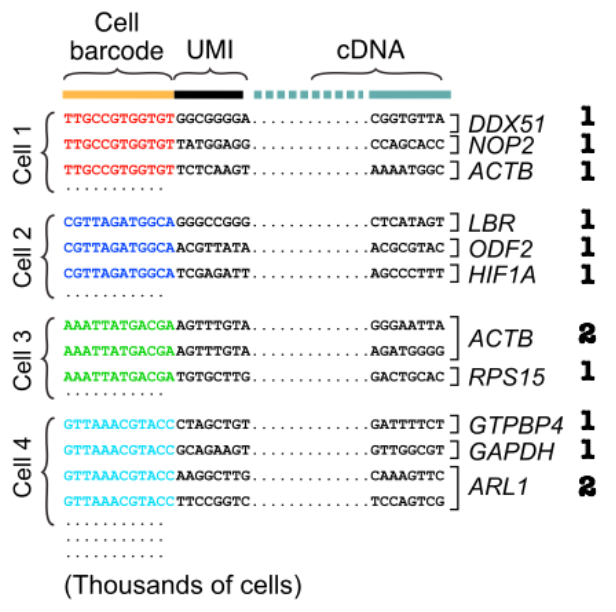
\includegraphics[width=8.56in]{_book/10X_files/figure-html/barcode}

\begin{verbatim}
**Quiz**
1. What is the difference between a cell barcode and UMI barcode? and what are their significance?
2. What are the lengths of the cell barcode and UMI barcode used in our dataset?
3. Are these barcodes located on the 5' or 3' read file?
\end{verbatim}

Generally 10X Genomics scRNA-Seq reads are aligned using the tool Cell Ranger. It is a wrapper to the open source alignment tool, STAR by Alexander Dobin, which optimises algorithms to handle the sequencing chemistry of 10X genomic library preparation. This includes UMI counting and calling cell barcodes. More information can be found at \url{https://support.10xgenomics.com/single-cell-gene-expression/software/pipelines/latest/algorithms/overview}.

In this workshop we will be using a recently developed application of STAR, STARsolo, which is an effective solution to handle droplet-based scRNA-seq data analysis. It provides an output similar to Cell Ranger which is important for downstream analysis packages such as Seurat. STARsolo also performs extremely fast read alignment of single cell raw reads from 10X genomics. It claims to be 10 times faster than Cell Ranger. More details can be found in the latest version of STAR manual: \url{https://github.com/alexdobin/STAR/blob/master/doc/STARmanual.pdf}.

Some of the key functions of STARsolo are:

\begin{verbatim}
1. Error correction and demultiplexing of cell barcodes using user-input whitelist.
2. Mapping the reads to the reference genome using the standard STAR spliced read alignment algorithm.
3. Error correction and collapsing (deduplication) of Unique Molecular Identifiers (UMIs).
4. Quantification of per-cell gene expression by counting the number of reads per gene.
\end{verbatim}

Create an output directory called ``starsolo\_out''.

\texttt{mkdir\ starsolo\_out}

Run the following command to perform read alignment:

\begin{verbatim}
STAR --genomeDir genome_index/ --soloType Droplet --soloCBwhitelist barcode_whitelist/10X_v2.txt --runThreadN 16 --readFilesCommand zcat --readFilesIn fastq/MelanomaT_CD45plus_IGO_07734_S5_L002_R2_001.fastq.gz fastq/MelanomaT_CD45plus_IGO_07734_S5_L002_R1_001.fastq.gz --outFileNamePrefix ~/starsolo_out/
\end{verbatim}

This step can take several minutes. Please work through the quiz questions in the meanwhile and ask questions!

\begin{verbatim}
**Quiz**
1. Describe the function of each parameter in the sequence alignment command.
2. What are some different types of scRNA-sequencing methods other than droplet based? And describe their differences.
\end{verbatim}

\hypertarget{starsolo-output}{%
\section{STARsolo Output}\label{starsolo-output}}

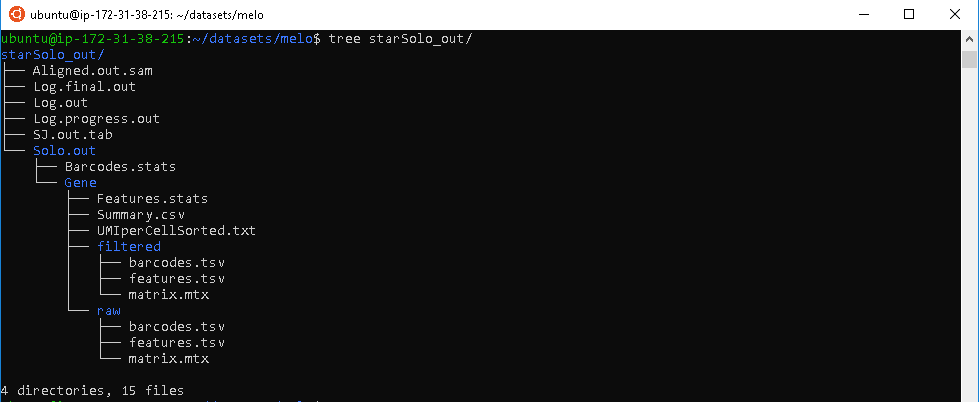
\includegraphics[width=9.79in]{_book/10X_files/figure-html/output}

The STARsolo program outputs a large amount of files reflecting details of the read alignment process. We will only discuss some of the key files important for downstream analysis.

\begin{enumerate}
\def\labelenumi{\arabic{enumi}.}
\tightlist
\item
  The \textbf{BAM file}, contains information about mapped reads, in a binary compressed format. When de-compressed into a SAM file, information is stored as a tab seperated table where the columns corresponds to:
\end{enumerate}

\begin{verbatim}
QNAME : read name (generally will include UMI barcode if applicable)
FLAG : number tag indicating the “type” of alignment, link to explanation of all possible “types”
RNAME : reference sequence name (i.e. chromosome read is mapped to).
POS : leftmost mapping position
MAPQ : Mapping quality
CIGAR : string indicating the matching/mismatching parts of the read (may include soft-clipping).
RNEXT : reference name of the mate/next read
PNEXT : POS for mate/next read
TLEN : Template length (length of reference region the read is mapped to)
SEQ : read sequence
QUAL : read quality
\end{verbatim}

BAM files can be viewed using SAMtools.

\texttt{samtools\ view\ output.bam}

\begin{enumerate}
\def\labelenumi{\arabic{enumi}.}
\setcounter{enumi}{1}
\item
  \textbf{Alignment summary} files, Features.stat and Summary.csv, contains information about basic mapping details. This can serve as an easy preliminary quality control check of the alignment process.
\item
  The \textbf{feature matrix} file, matrix.mtx, contains information about the counts of genes mapped in each individual cell. The column names corresponds to each individual cell barcode, and the row names corresponds to all annotated genes. Due to the large size of this data, it is stored as a sparse matrix.
\item
  \textbf{Auxiliary files}, barcodes.tsv and features.tsv, provide extra metadata important for downstream analysis. These files along with the matrix file are required for analysis in gold standard scRNA-seq data analysis package, seurat.
\end{enumerate}

\hypertarget{scrna-seq-downstream-analysis}{%
\chapter{scRNA-seq Downstream Analysis}\label{scrna-seq-downstream-analysis}}

\hypertarget{seurat-package}{%
\section{Seurat Package}\label{seurat-package}}

Seurat is an R package designed for QC, analysis, and exploration of single-cell RNA-seq data. Seurat aims to enable users to identify and interpret sources of heterogeneity from single-cell transcriptomic measurements, and to integrate diverse types of single-cell data.

The format of output results from both Cell Ranger and STARsolo stream nicely into the Seurat defualt analysis pipeline. We will not demonstrate this process but only highlight the types of insights/plots you can achieve from this data analysis. More information can be found at \url{https://satijalab.org/seurat}.

\hypertarget{differentially-expressed-genes}{%
\subsection{Differentially expressed Genes}\label{differentially-expressed-genes}}

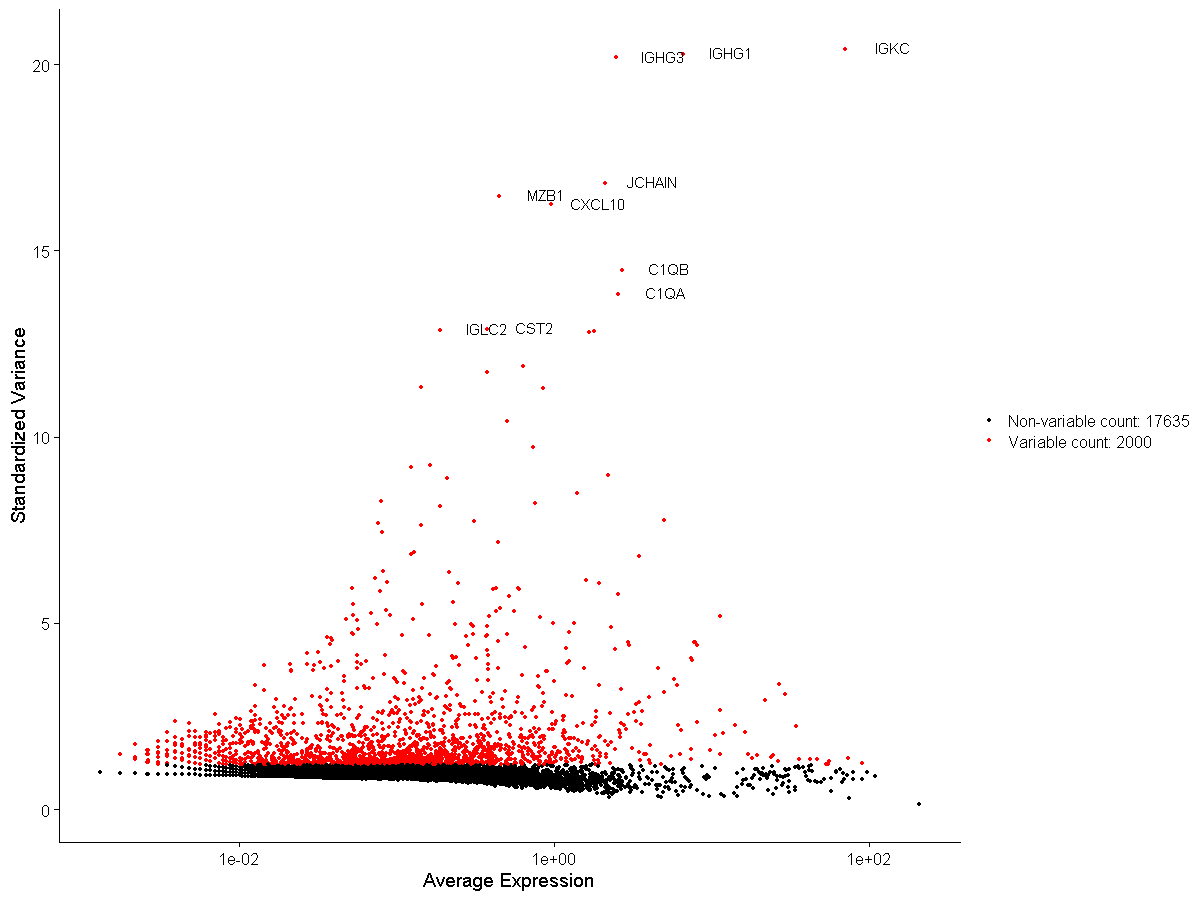
\includegraphics[width=16.67in]{_book/10X_files/figure-html/differential_genes}

\hypertarget{cell-clustering}{%
\subsection{Cell Clustering}\label{cell-clustering}}

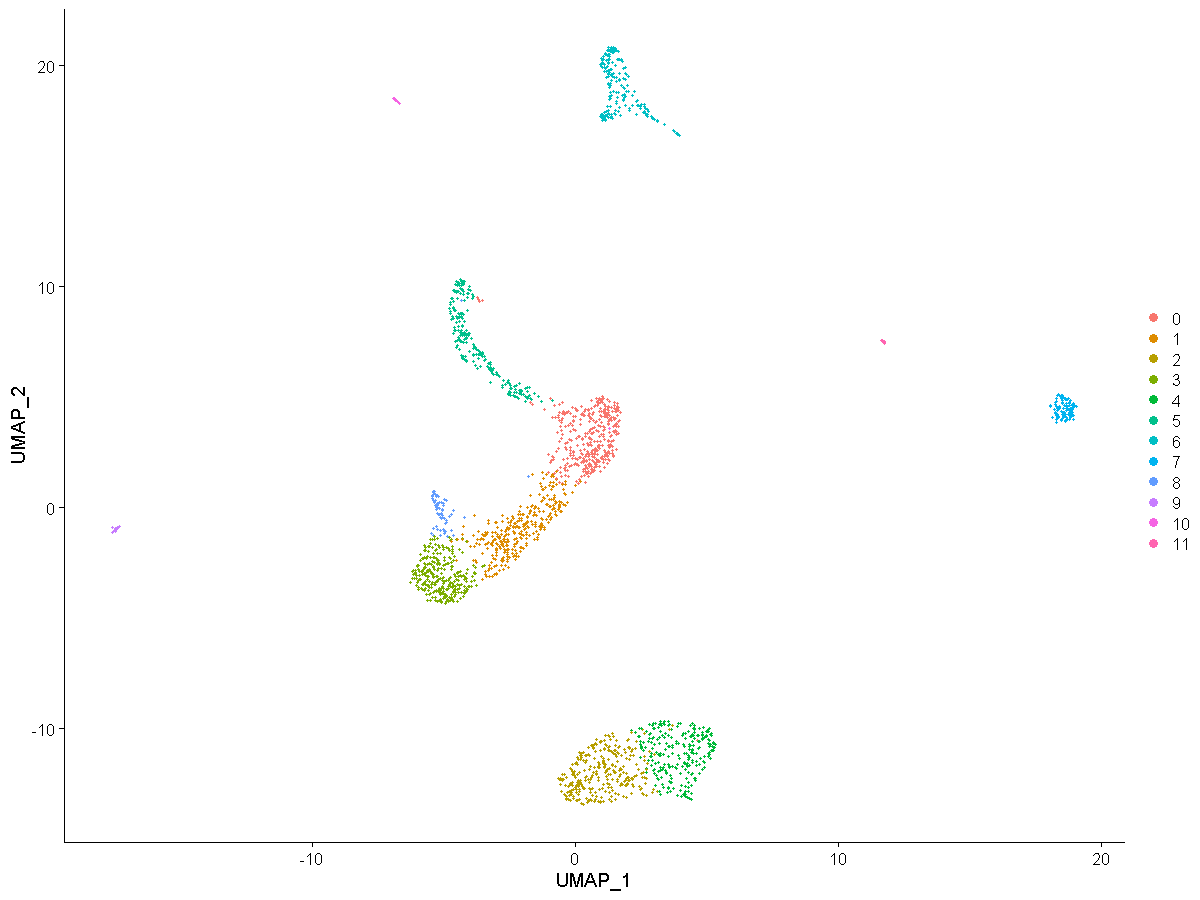
\includegraphics[width=16.67in]{_book/10X_files/figure-html/UMAP}

\hypertarget{analysis-of-variable-gene-markers}{%
\subsection{Analysis of Variable Gene Markers}\label{analysis-of-variable-gene-markers}}

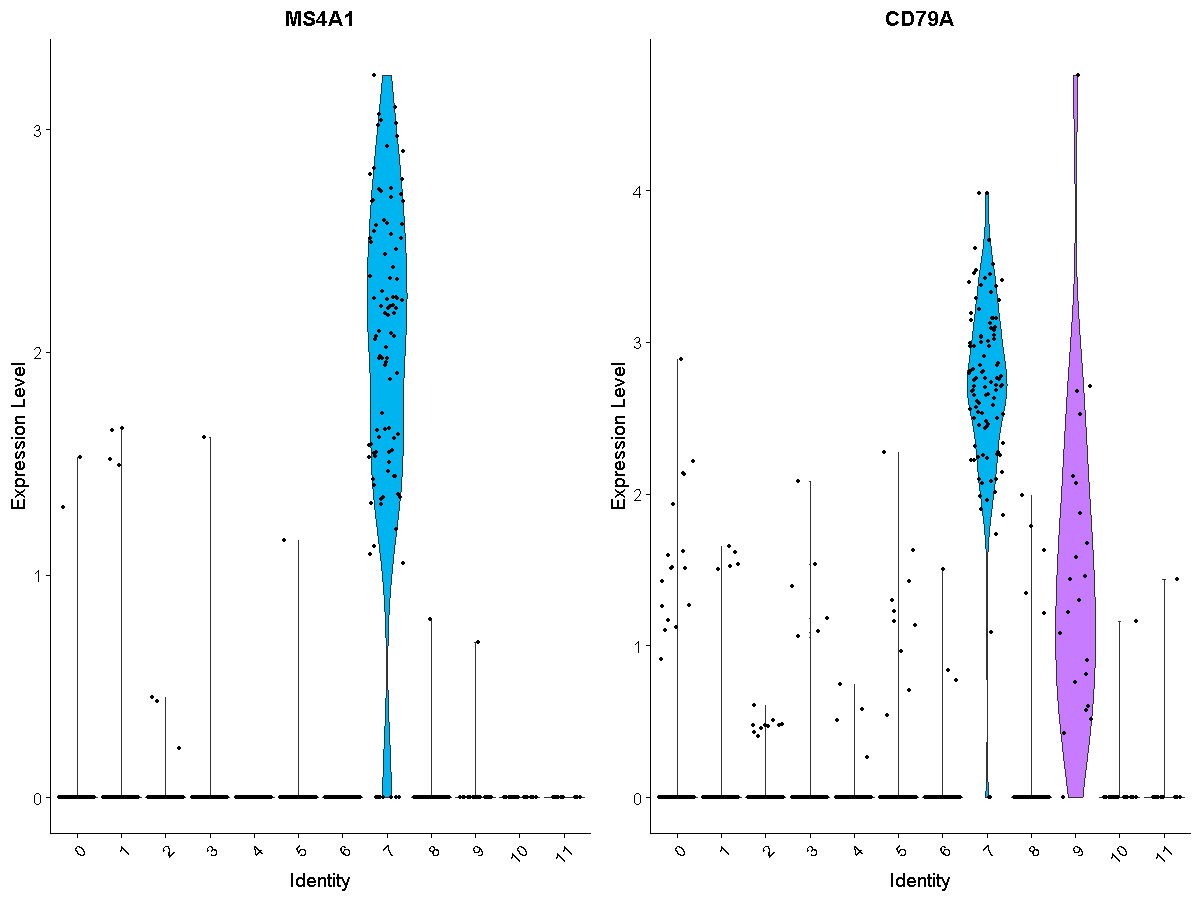
\includegraphics[width=16.67in]{_book/10X_files/figure-html/gene_markers}

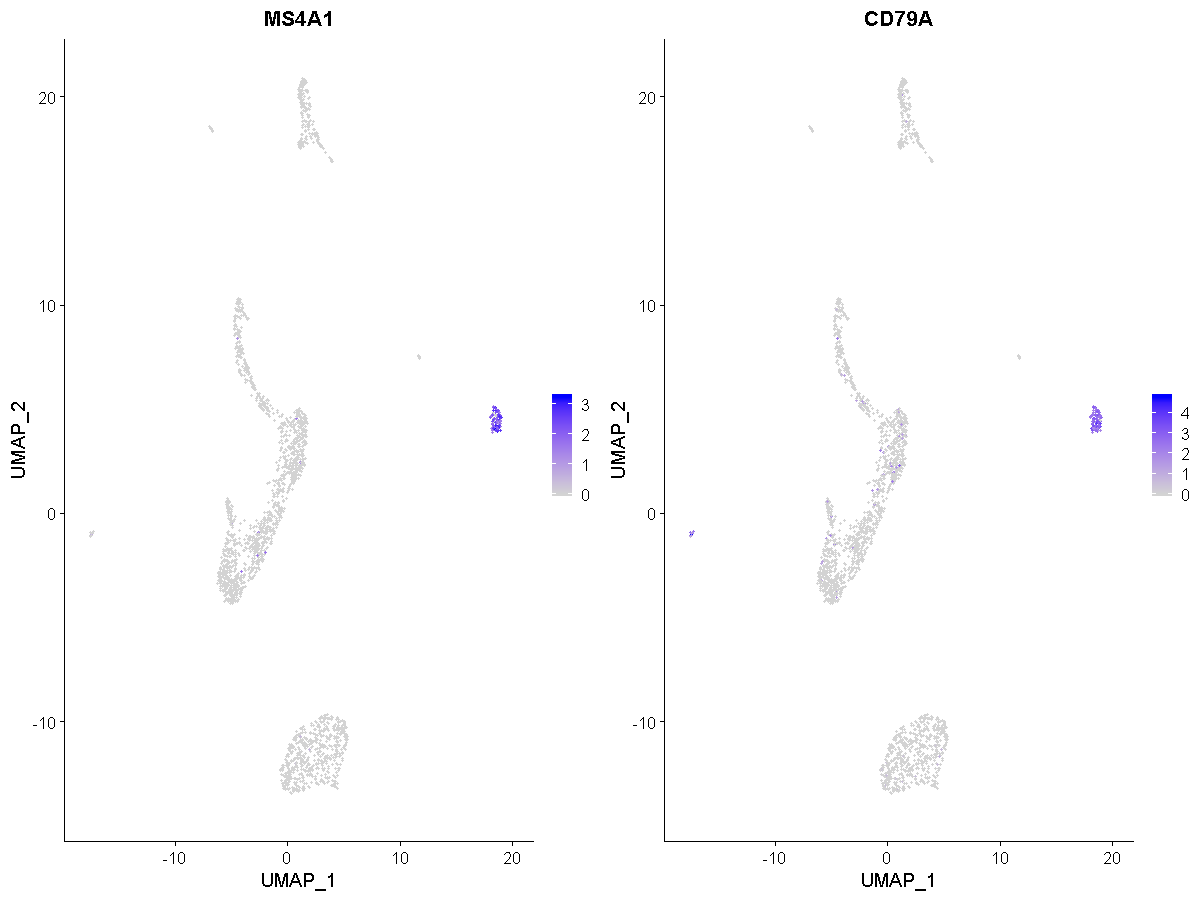
\includegraphics[width=16.67in]{_book/10X_files/figure-html/gene_markers2}

\hypertarget{heatmap-of-gene-expression-by-clusters}{%
\subsection{Heatmap of gene expression by clusters}\label{heatmap-of-gene-expression-by-clusters}}

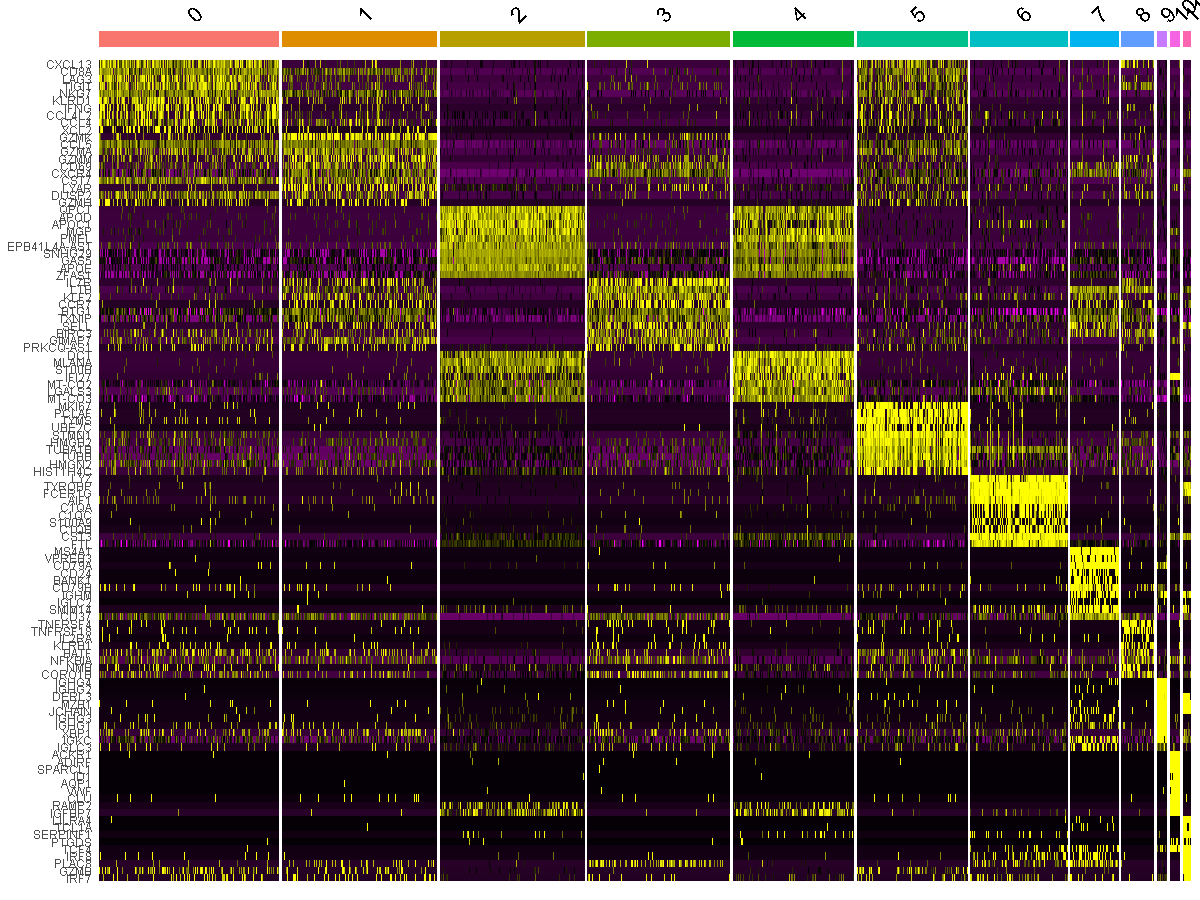
\includegraphics[width=16.67in]{_book/10X_files/figure-html/heatmap_clusters}

\hypertarget{references}{%
\chapter{References}\label{references}}

Dobin, A., Davis, C. A., Schlesinger, F., Drenkow, J., Zaleski, C., Jha, S., \ldots{} Gingeras, T. R. (2013). STAR: Ultrafast universal RNA-seq aligner. Bioinformatics, 29(1), 15--21. \url{https://doi.org/10.1093/bioinformatics/bts635}

\bibliography{book.bib,packages.bib}


\end{document}
